\documentclass[11pt,a4paper]{article}
\usepackage{amsmath}
\usepackage{amsfonts}
\usepackage{amssymb}
\usepackage{fullpage}
\usepackage{graphicx}
\usepackage{hyperref}
\usepackage{float}
\usepackage{siunitx}
\usepackage{mathrsfs}
\usepackage{subcaption}
\usepackage{ulem}
\usepackage{xcolor,cancel}
\usepackage{tikz}
\usetikzlibrary{shapes.geometric, arrows}
\tikzstyle{startstop} = [rectangle, rounded corners, minimum width=3cm, minimum height=1cm,text centered, draw=black, fill=red!30]
\tikzstyle{io} = [trapezium, trapezium left angle=70, trapezium right angle=110, minimum width=3cm, minimum height=1cm, text centered, draw=black, fill=blue!30]
\tikzstyle{process} = [rectangle, minimum width=3cm, minimum height=1cm, text centered, draw=black, fill=orange!30]
\tikzstyle{decision} = [diamond, minimum width=3cm, minimum height=1cm, text centered, draw=black, fill=green!30]
\tikzstyle{arrow} = [thick,->,>=stealth]
\newcommand\hcancel[2][black]{\setbox0=\hbox{$#2$}%
\rlap{\raisebox{.45\ht0}{\textcolor{#1}{\rule{\wd0}{1pt}}}}#2}

\begin{document}
	\title{Numerical and Computational method in Research - PYL800\\
	Assignment - 3}
	
	\author{Apoorav Singh Deo\\
	2021PHZ8046}
	\maketitle




\section{Problem Statement}
Write a program to simulate 2-dimensional Rutherford back scattering experiment, with the incoming particle having a Gaussian profile. Convert the uniform distribution to Gaussian distribution for this problem. 

Plot the fraction of scattered particles as a function of the standard deviation $\sigma = 0.1, 0.5, 1, 5$ of the Gaussian profile?

\section{Generation of Random Numbers}
For this code random numbers are generated using \texttt{random()} which is included by default in a standard python package. Only thing one has to do is just include the random package in our code.

Functions in the random module rely on a pseudo-random number generator function known as \textbf{Mersenne Twister PRNG algorithm}. These types of function does not produce actual random numbers but they do the job well.

\section{Generating Gaussian Type Random Numbers}
A Gaussian function is given by the equation (\ref{eq_1})

\begin{align}\label{eq_1}
p(x) = \frac{1}{\sqrt{2\pi\sigma^2}}\ e^{-\left[\frac{x^2}{2\sigma^2}\right]}
\end{align}

Here in our case we need to generate two set of random numbers, As in code it is given by \texttt{x1} and \texttt{y1}\footnote{\texttt{z1} is also seen in the code. \texttt{z1} is used only for debugging purpose.}. The whole exercise of generating the random numbers is done in polar coordinate system. 

We have two independent random numbers \texttt{x1}, \texttt{y1}, both are drawn form the Gaussian distribution with the same standard deviation $\sigma$ (the values of $\sigma$ is given in the question). The probability that the point with position vector (\texttt{x1}, \texttt{y1}) falls in some element $dx\ dy$ of the $x-y$ plane is given by:

\begin{align*}
p(x)\ dx \times p(y)\ dy &=  \frac{1}{\sqrt{2\pi\sigma^2}}\ e^{-\left[\frac{x^2}{2\sigma^2}\right]}\ dx \times \frac{1}{\sqrt{2\pi\sigma^2}}\ e^{-\left[\frac{y^2}{2\sigma^2}\right]}\ dy \\
&= \frac{1}{2\pi\sigma^2}\ e^{-\left[\frac{x^2+y^2}{2\sigma^2}\right]}
\end{align*}

Now working out the polar conversion, where $x^2 + y^2 = r^2$ and surface element is defined as, $r\ dr d\theta$. Therefore, we get

\begin{align*}
p(r)\times p(\theta)\ dr\ d\theta = \left(\frac{r}{\sigma^2}\right) \ e^{-\left[\frac{r^2}{2\sigma^2}\right]}dr \times \frac{d\theta}{2\pi} 
\end{align*} 

Generating the $\theta$ variable is trivial - the distribution $p(\theta) = 1/2\pi$ is just a uniform distribution, so all what is to be done is to produce random number between zero and $2\pi$. The radial coordinate $r$ can be generated using the transformation method. Therefore,

\begin{align*}
p(r) &= \frac{r}{\sigma^2}\ e^{-\left[\frac{r^2}{2\sigma^2}\right]}
\end{align*}

Integrating the above equation using appropriate limits (\textit{z} is the place where \texttt{random()} is used to generate random number, where it varies from 1 to 0), we get:

\begin{align*}
r = \sqrt{-2\sigma^2\ln(1-z)}
\end{align*}

With the value for $r$ and our random value for $\theta$, our two Gaussian random numbers are given by converting back to Cartesian coordinates thus,

\begin{align*}
x = r\cos(\theta)\ &\ y = r\sin(\theta)
\end{align*}

A Gaussian beam with $\sigma = 0.5\times \frac{a_0}{100}$, where $a_0$ is Bohr's radius [Figure(\ref{fig_1})]

	\begin{figure}[H]
	\begin{center}
	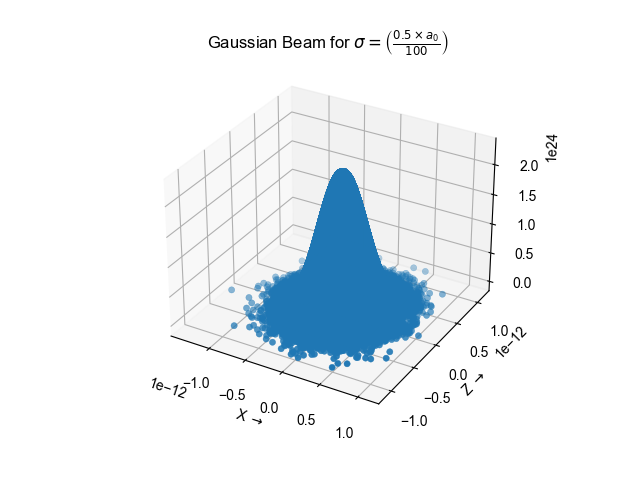
\includegraphics[width=0.7\textwidth]{Figure_1.png}
	\caption{Gaussian beam.}
	\label{fig_1}
	\end{center}
	\end{figure}
	
\section{Rutherford Scattering Simulation}
In the last section, algorithm is known to generate two independent random numbers to fit the Gaussian scheme. Now we need to begin the actual simulation.

	\begin{figure}[H]
	\begin{center}
	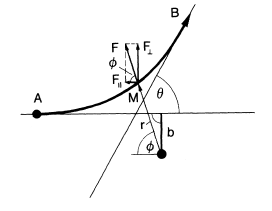
\includegraphics[width=0.4\textwidth]{rf.png}
	\caption{Rutherford Scattering}
	\label{fig_3}
	\end{center}
	\end{figure}

$b$ parameter is only thing we need to check in out iteration. It is also known as distance of closest approach. Also, shown in Figure (\ref{fig_3})

\begin{align}\label{eq_2}
b = \frac{Ze^2}{2\pi\epsilon_0E}
\end{align}
Here, Z = 79 i.e. Gold and energy of the alpha particle beam is taken as 7.6 MeV. Rest other constant hold their values in SI units.\medskip


In the code it is to specified that point generated should be closer to the gold atom's nuclei. The distance is less than $b$.

\begin{align*}
\sqrt{x1^2 + y1^2} < b
\end{align*}

\section{Result}
File enclosed with the report \begin{verbatim}
assignment_3_code.py
\end{verbatim}

\noindent Contains the code for this job. Final graph generated keeping $N=10^5$. This number can be changed inside the code and result could be checked for higher values as well as lower values of the $N$. The graph in Figure (\ref{fig_2}) shows the change reflected particles with change in the size of the Gaussian beam.\medskip

\noindent \textbf{Note: } To generate meaningful results the $\sigma$ value of the Gaussian curve is scaled by the factor of $a_0/100$. There is no hard and fast rule for taking such value but only thing is to be kept in mind is that b is of the order of $10^{-14}$ for which Gaussian beam of even order $0.1$ is useless. Rather, $a_0/100$ just scaled the $\sigma$ suggested in the question.

	\begin{figure}[H]
	\begin{center}
	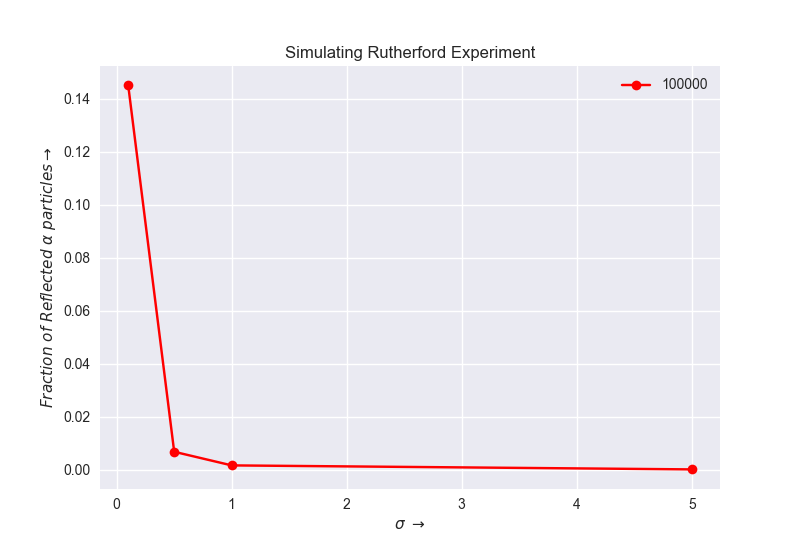
\includegraphics[width=0.8\textwidth]{Figure_2.png}
	\caption{Fraction of Reflected $\alpha$ particles versus $\sigma$ of Gaussian Beam.}
	\label{fig_2}
	\end{center}
	\end{figure}
	
Excerpt from the Command-line
\begin{verbatim}
Running simulation for Sigma value 0.1
Generating Random Number Stream . . . 
14409.0 particles were reflected back out of 100000
Simulation Done!

---------------------------------------------

Running simulation for Sigma value 0.5
Generating Random Number Stream . . .
606.0 particles were reflected back out of 100000
Simulation Done!

---------------------------------------------

Running simulation for Sigma value 1.0
Generating Random Number Stream . . .
179.0 particles were reflected back out of 100000
Simulation Done!

---------------------------------------------

Running simulation for Sigma value 5.0
Generating Random Number Stream . . .
7.0 particles were reflected back out of 100000
Simulation Done!
\end{verbatim}
	
\section{Code Execution}

\noindent [\texttt{For Windows and Mac}] Anaconda distribution\footnote{\url{https://www.anaconda.com/products/individual}} don't need any dependencies to be installed. One can simply run the code in it using any one of the IDEs in it. (Spyder is suggested).\medskip

\noindent [\texttt{For Linux}] Terminal can also be used to execute this code, but make sure dependencies are installed before hand. These dependencies can be installed using  \texttt{pip}.\footnote{\url{https://pip.pypa.io/en/stable/}}. Type in these commands in the BASH terminal after installing pip.

\begin{enumerate}
\item \texttt{pip install matplotlib}
\item \texttt{pip install numpy}
\item \texttt{pip install scipy}
\end{enumerate}

To execute the program run command on the BASH terminal:
\begin{verbatim}
>> python3 file_name.py
\end{verbatim}

\section{References}

\begin{enumerate}
\item [Docs:] \url{https://docs.python.org/3/library/random.html}
\item [Book:] Computation Physics by Mark Newman.
\end{enumerate}

\section{Code}
\begin{verbatim}
# -*- coding: utf-8 -*-
"""
Created on Sat Oct 30 14:29:45 2021

@author: Apoorav Singh Deo (Enrollment Number: 2021PHZ8046) 

Intended to compelete the course requiremnt of PYL800 - 

Numerical and Computational method in Research

Do not distribute.
"""

import random 
# Importing Random to generate random number
import math
# Importing math modules to access mathematical Functions
from matplotlib import pyplot as plt
# Importing matplotlib for plotting the graphs
import numpy as np
# Importing numpy module to access faster arrays

sgm = np.array([0.1, 0.5, 1, 5])
# Defining sigma values as mentioned in the question

#sgm = np.linspace(0.1,5,100)

ite_len = len(sgm)
# It calculates the array size of input sigma value (Helpful in iteration)




# Defining the Gaussian Function [For Debugging only]

def gaussian(sigm, x, y):

# sigm is the sigma value of the gaussian function
# x is the argument of the function

    g_f = 1/(2*math.pi*sigm**2)*math.exp(-(x*x + y*y)/(2*sigm**2))
    
# "g_f" is the return variable with parameters for gaussian function
    
    return g_f

N = 10**5
# Number of alpha-particle bobarded towards the atom
Z = 79
# Atomic number of the Gold atom [amu] 
e = 1.602e-19
# Electronic Charge [C]
E = 7.7e6*e
# Energy of incoming alpha particle [eV] ==> [J]
eps_0 = 8.854e-12
# Constant \epsilon_0 [SI]
a0 = 5.292e-11
# Bohr Radius [SI]

# Gaussian Type Random number Generator Function
def g_R(sigm):

# "sigm" is the sigma value of the Gaussian Function
 
    r = math.sqrt(-2*sigm**2*math.log(1-random.random()))
# Generation of radom radial points
    theta = 2*math.pi*random.random()
# Generation of Random \theta values 
    x = r*math.cos(theta)
# Building x - co-ordinate out of the random values
    y = r*math.sin(theta)
# Building y - co-ordinate out of the random values
    return x,y
# Return Function

x1 = np.empty([N,ite_len])
y1 = np.empty([N,ite_len])
z1 = np.empty([N,ite_len])
# Decalaring two dimensional array (z1 is declared for debugging purposes) 
# Numpy array is declared 

k = 0
# Used for indexing cnt[] 

cnt = np.empty(ite_len)
# Declaring the "cnt" variable to count the atoms reflected back


for j in sgm:
    
    print("Running simulation for Sigma value {}".format(j))
    
    cnt[k] = 0
    # Setting value to zero to avoid garbage values.

    b_par = (Z*e*e/(2*math.pi*eps_0*E))
    # Parameter declaration: Distance of Closest Approach

    #print(b_par)
    print("Generating Random Number Stream . . . ")
    for i in range(N):
        x1[i,k],y1[i,k] = g_R(j*a0/100)
        # Initializing the function for random number generation
        z1[i,k] = gaussian(j*a0/100, x1[i,k], y1[i,k])
        # For debugging purpose only
        b = math.sqrt(x1[i,k]*x1[i,k]+y1[i,k]*y1[i,k])
        # Pin pointing data value
        #print(b)
        if (b < b_par):
            cnt[k] += 1
    
    print("{} particles were reflected back out of {}".format(cnt[k], N))
    print("Simulation Done!")
    print("\n---------------------------------------------\n")
    k += 1
    # Iteration finishes
        
            

#---------------------
# Plotting
plt.style.use('seaborn')    
plt.plot(sgm, cnt/N, "r-o", label=str(N))
plt.xlabel(r"$\sigma\ \rightarrow$")
plt.ylabel(r"$Fraction\ of\ Reflected\ \alpha\ particles \rightarrow$")
plt.legend()
plt.title("Simulating Rutherford Experiment")
plt.grid(1)
plt.show()
\end{verbatim}
\end{document}
